\section{Theoretical Framework}
In order to thoroughly understand the aim and subject of the report, it is important to explore different existing solutions and literature. Therefore, the subjects that will be discussed in the following theoretical framework are Cloud Streaming/Cloud Computing, Virtual Reality and Security in a streaming context. Within this theoretical framework definitions of the subjects will be given, as well as current insights into these subjects. The topics reflect knowledge needed to understand the problem space. Together all of the topics make up the 360 scan. Then this knowledge will be applied to the research problem by creating an overview of the individual parts of a cloud \acrshort{vr} system and of the available components to create one. 
\subsection{Cloud Streaming/Cloud Computing}

\subsubsection{Definition}
According to Armbrust et al. (2010) Cloud computing is defined as follows: 
"Cloud computing refers to both the applications delivered as services over the Internet and the hardware and systems software in the data centres that provide those services." \parencite{aviewoncc}
We can then further define Cloud streaming as the applications that are delivered over the internet as a service.

\subsubsection{Existing Solutions and Technology}
Several commercial gaming cloud streaming services already exist, such as Google Stadia \parencite{stadia}, XBox XCloud \parencite{xcloud} and Nvidia GeForceNow \parencite{geforcenow}. These applications deliver conventional games from a powerful computer in a server to the client device at home. Despite initial setbacks, cloud streaming is now a mainstream technology. The start of 2020 also saw the first experimental cloud \acrshort{vr} streaming development kits, such as Nvidia's CloudXR \parencite{cloudxr}, and closed beta's for commercial cloud \acrshort{vr} streaming services \parencite{shadowvr} (Available on Windows, macOS, Ubuntu, Android and iOS) . Additionally the first commercial retail product with cloud \acrshort{vr} has been released \parencite{zerolight5g}, however it runs on custom made \acrshort{hmd}'s and not on consumer platforms . There is also a variety of Infrastructure\hyp{}as\hyp{}a\hyp{}service (IaaS) platforms, such as Amazon's AWS \parencite{aws}, Microsoft's Azure \parencite{azure} and Google's Cloud Platform \parencite{gcp}, that provide generic computing power and storage in a cloud computing/streaming context.
%Maybe remove survey since it is 5 years old
 These services generally cannot achieve the \hyperref[ssec:vrphy]{latency requirements} of cloud \acrshort{vr} streaming \parencite{survey_IRSS} as it requires an extraordinarily low latency of $>$20\acrshort{ms} from \acrfull{mtp}, where most (game) streaming applications have a higher tolerance for latency. Some companies actively develop technology to minimize latency exactly for purposes like this (e.g. enabling compute power as physically close to the end user as possible \parencite{awswavelength}, but generally as time and technology progress the capabilities of cloud streaming services will grow alongside.

\subsubsection{System Architecture types (for a cloud VR system)}
\begin{figure}[h]
\caption{Cloud Server, Remote Edge, Local Edge visualized \parencite{wlanvr}}
\label{fig:arch1}
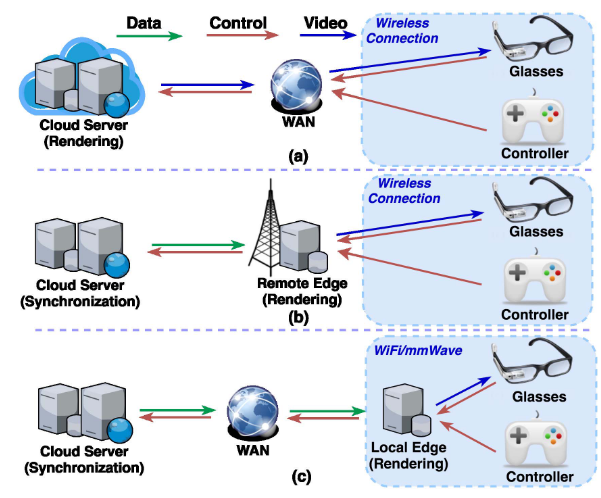
\includegraphics[scale=0.45]{Architectures1}
\end{figure}

One of the main considerations when designing a cloud \acrshort{vr} streaming application is the decision to either use a Cloud, Remote Edge or Local Edge computing device for the rendering of the frames (See \hyperref[fig:arch1]{Figure 1} and \cite{wlanvr}):
\begin{itemize}
\item A cloud server renders the \acrfull{fov} (current view) remotely and streams the corresponding video to the user’s \acrfull{hmd}. 
\item A Remote Edge sever receives information about the context from a  cloud server, renders the appropriate frame and streams the video to the user’s \acrshort{hmd}. The main advantage here is that edge servers are located closer to the end user (thus improving response time and saving bandwidth)
\item A Local Edge server receives compressed models as well as textures, renders it locally and streams the video to the user’s \acrshort{hmd}.
\end{itemize} 

\begin{figure}[h!]
\caption{Example System Architecture}
\label{fig:sysarch}
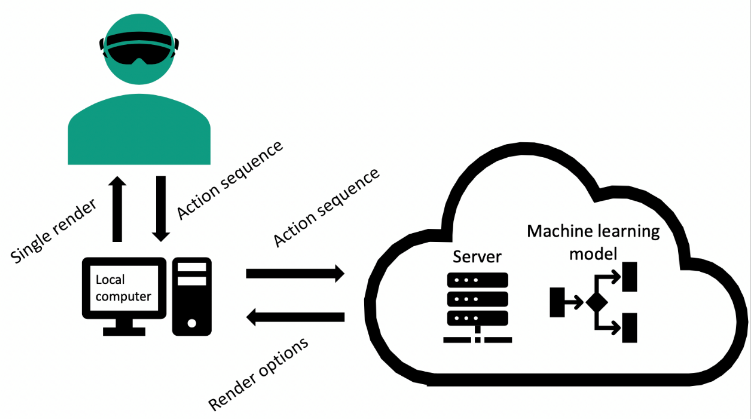
\includegraphics[scale=0.45]{SimpleArchitecture}
\end{figure}

For the purposes of this research I will ignore Local Edge system architectures. The reason is that one of the major motivations for this report was the desire to keep data as safe as possible, which in this case means keeping in the cloud. A Local Edge system, by design, requests and receives business data to render the frame for the user locally. For this reason a Local Edge approach would be the wrong direction to research in. An example architecture of a cloud \acrshort{vr} solution that keeps the business data in the cloud can be seen in \hyperref[fig:sysarch]{Figure 2}.

Furthermore one also has to consider if the application will be hosted on a cloud service provider or on an in-house server. Both ways have advantages and disadvantages, which are elaborated upon in the \nameref{sec:app}, and the decision should be made based on the unique circumstances of each customer.

\subsubsection{Latency}
The most important metric for a system architecture is the latency between the user input, such as movement of the \acrshort{hmd}, and the updated frame appearing on the users display. Recent measurements of cloud gaming services measure this latency at between 135 and 240\acrshort{ms} \parencite{lagmeasure}. This is acceptable for most games, except maybe high intensity reaction games. \acrshort{vr} unfortunately has severely stricter latency requirements, which are elaborated upon in \nameref{ssec:vrphy}

\subsection{Constraints of Virtual Reality}
\label{ssec:vrphy}
As mentioned before, when developing a \acrshort{vr} application, there are a few physical constraints that developers need to be aware of. The most important threshold to know is the 20\acrshort{ms} \acrshort{mtp} delay. Upon input from the \acrshort{hmd}, the developer has to display a new rendered image within an average of 20\acrshort{ms} to avoid motion sickness for users. The more this threshold can be undercut, the better the chances to have an acceptable gameplay experience without motion sickness. Interaction input, such as the input from the controllers, can safely be processed at delays of $>$100\acrshort{ms} without any negative repercussions in terms of \acrfull{qoe}.

\subsection{Security (for streaming data)}
From a technical standpoint there are 2 major categories of security implementations: Encryption and Access management. There are additional measures that companies can take such as having consistent security protocols and educating employees, but for this report the focus is on technical solutions:

\subsubsection{Encryption}
Encryption is the practice of scrambling data so that unauthorized users cannot use the data. Only an authorized party in possession of the decryption key can un-scramble the data and subsequently use it. 
One such encryption technologies is the \acrfull{aes}, which comes with three different key sizes: 128, 192 and 256 bits. In 2016 it was estimated that it would take 500,000,000,000 years to decrypt just one \acrshort{aes}-128 key.
To encrypt the data in delivery, a technology such as the \acrfull{tls} can be used, which encrypts the data based on a shared secret that was negotiated at the start of the session, thus making the data only usable for the server and client who have the decryption key.
\subsubsection{\acrfull{iam}}
An \acrshort{iam} solution tracks users and what they are allowed to do. There are multiple existing solutions for tracking the users privileges, but for this report only cloud based services are relevant since the premise of this research is the ability to have a cloud solution. All major cloud providers have \acrshort{iam} solutions in their ecosystem and in case of a in-house server a independent \acrshort{iam} service provider can satisfy that requirement.

\subsubsection{Latency Implications}
As discovered by existing research, encryption does not greatly influence performance of the video stream in terms of latency \parencite{Kaknjo_2019}.

\newpage
\subsection{Components of a cloud \acrshort{vr} pipeline}
In this section all the individual components of a cloud \acrshort{vr} pipeline are being presented. Furthermore an overview of pre-made components will be presented and which part of the pipeline they address.

\begin{figure}[h!]
\caption{Overview of components in a typical cloud \acrshort{vr} pipeline}
\label{fig:pipeline}
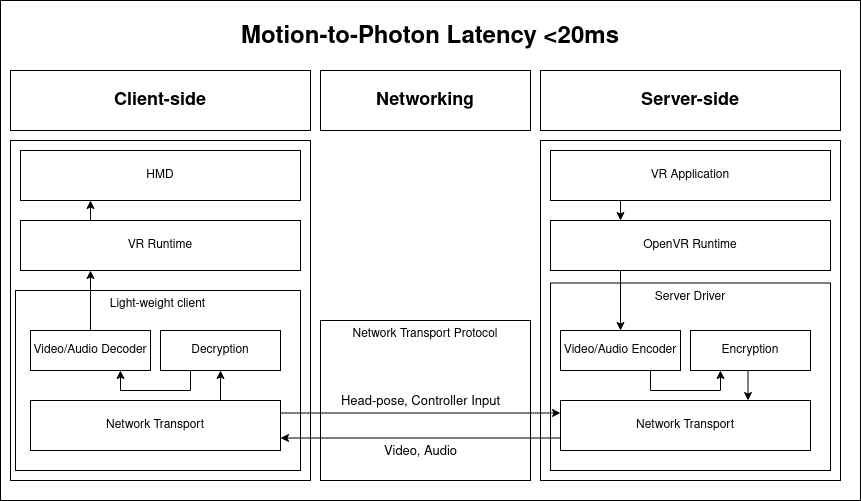
\includegraphics[scale=0.4]{CloudVR_PipelineComponents}
\end{figure}

%WRITE DOWN HOW MUCH TIME IN ms EACH STEP TAKES

\paragraph{\textSR}
The actual \acrshort{vr} application will be running on the cloud server and use the servers hardware to render the game. The application will be running on the OpenVR SDK, which allows access to VR hardware from multiple vendors without requiring that applications have specific knowledge of the hardware they are targeting \parencite{openvrsdk}. 
\paragraph{\textSECO}
The rendered frames will be encoded with a video compression codec before they are sent to the networking layer.
\paragraph{\textSECR}
Before transmitting the data (encoded frames) over the network it will be encrypted to maximise security.
\paragraph{\textN}
Through the network connection both the output (rendered, encoded and encrypted frames) and the input (\acrshort{hmd} position and controller input) will be exchanged between the server and the client.
\paragraph{\textCDCR}
Once received from the networking layer, the frames are decrypted to prepare for decoding.
\paragraph{\textCDCO}
Once decrypted to usable packages, the data will be decoded and then sent to the VR Runtime
\paragraph{\textCRD}
The decoded frames will be warped to fit the lenses of the \acrshort{hmd} and then finally be displayed to the user.


\subsubsection{Available components}
\renewcommand{\arraystretch}{1.5}

%Perhaps accompany with a color coded image
\begin{longtable}{  | p{0.15\linewidth} | p{0.5\linewidth} | p{0.35\linewidth} | }
\caption{Available Components} \\
\hline
\textbf{Name} & \textbf{Description} & \textbf{Solves} \\ 
\hline
NVIDIA CloudXR SDK & "NVIDIA CloudXR™, a groundbreaking technology built on NVIDIA RTX™, delivers VR and AR across 5G and Wi-Fi networks. With NVIDIA GPU virtualization software, CloudXR is fully scalable for data center and edge networks" \parencite{cloudxr}. & \textSECO , \textSECR ,  \textN , \textCDCR , \textCDCO , \textCRD \\
\hline
Seurat & Seurat is a system for image-based scene simplification for VR. It converts complex 3D scenes with millions of triangles, including complex lighting and shading effects, into just tens of thousands of triangles that can be rendered very efficiently on 6DOF devices with little loss in visual quality \parencite{seurat}. & \textSR  \\
\hline
H.264 & H.264 is a video compression standard based on block-oriented, motion-compensated integer-DCT coding.[1] It is by far the most commonly used format for the recording, compression, and distribution of video content. It supports resolutions up to and including 8K UHD. & \textSECO , \textCDCO \\
\hline
VP8 & VP8 is an open and royalty free video compression format.  & \textSECO , \textCDCO \\
\hline
\acrfull{aes}  & \acrshort{aes} is a specification for the encryption of electronic data. & \textSECR , \textCDCR \\
\hline
\acrfull{tls} & \acrshort{tls} is a cryptographic protocol designed to provide communications security over a computer network by utilizing the \acrshort{aes} technology. & \textSECR , \textCDCR , \textN \\
\hline
WebRTC & With WebRTC, you can add real-time communication capabilities to your application that works on top of an open standard. It supports video, voice, and generic data to be sent between peers, allowing developers to build powerful voice- and video-communication solutions. The technology is available on all modern browsers as well as on native clients for all major platforms \parencite{webRTC}. & \textN \\
\hline
WebXR & The WebXR Device API provides the interfaces necessary to enable developers to build compelling, comfortable, and safe immersive applications on the web across a wide variety of hardware form factors. & \textSR , \textCRD \\
\hline
\end{longtable}